% {\color{red}asdf}

\newtheorem{DEF}{Definition}

%=====================================================================================
\chapter{Introduction}
%=====================================================================================

In these days, Continuous Integration (CI) is more often used in larger projects, where multiple developers are working on one and the same software product. This process ensures fast software development, called eXtreme Programming (XP), known as agile software development methodology. The methodology is mainly used to accelerate the development, nevertheless, development of software may be disrupted in various other ways. Nowadays, although this type of software development has many disadvantages, it is still much more often used on larger projects. The progress of the development may not be reached with a continuous integration which guarantees less disorder and failures. You may also know that the continuous integration is a part of the following open-source projects e.g. Facebook, Twitter, Mozilla. These projects use one of many famous continuous integration service Travis CI. Excluding Travis CI, there are plenty of other continuous integration services you may heard about, such as Jenkins, TeamCity, CircleCI, GitLab CI, Codeship and so on.\\

The software development process requires many code checking tools after every single code change in the source code. For as much as with every single change of code, there is a possibility to add, fix, derange or deteriorate any parts of the software product. These tools provide an automated code review and they afford a quick feedback by which they try to prevent these code impairments. Feedback about his adjustment is sent to the developer, who has made the change in the code. The automated process which provides the code review does not bother with executing a huge amount of tests. Above mentioned process is conducted via continuous integration server, which compiles the code, runs scripts and tests. The results are aggregated and the feedback is given to the developer who has made this code change. Continuous integration server is invoked every single time after any change is fetched in the source code and he had to execute the stated acts which are predefined. In next chapters we describe in details how does this workflow work and what steps are required to run.\\

The essence of this work is about the basics of continuous integration and its fundamentals. This thesis attempts to explain how the fundamentals of continuous integration and automated code review work. It describes how it is integrated to the software development, and how it works on an extensive project nowadays. Examples will be based on open-source project e.g. ManageIQ, which is a cloud manager founded by RedHat. The development process of the ManageIQ rests in agility and stability of the progress. These main factors of the development process could not be reached without a quick feedback to the developers working on project about their changes, that are submitted to the software product.

%=====================================================================================
\chapter{Continuous Integration and Automated Code Review}
%=====================================================================================

In the face of the fact that continuous integration and automated code review are used in a lot of projects, it is still an unknown part of software development. Despite CI rising as a big success story in automated software engineering, it has received almost no attention from the research community\cite{COPE}. There are only a few researches describing this part of development how is it deployed, managed and used. Development analysts are not giving an adequate attention to this part of software development. They are usually describing it as a common part of development in a software development process. This part is concerning to extreme programming due to fast code change deployment. This development technique is very adaptive and still more and more open source projects are using it. There are many developers relying on this type of software development which helps them rapidly. This chapter will give you a detailed view of the modern in-use software development methodology which is still in evolution.

%=====================================================================================
\section{Continuous Integration}
%=====================================================================================

Continuous integration (CI) has a key role in the software development process consisting of a few certain unavoidable steps which will be described later in next subsections. Everything begins at the moment, when one developer who has made changes in a source code of the software product is trying to commit them into the software product. The process of continuous integration has begun at this point and lasts until feedback is sent back to the developer. These stages of continuous integrations are proceed every time after the CI server has detected a change in a version control repository. This automation has a lot of benefits which are necessary to keep the software product without any kind of defects. Many of them are detected in time and reported back to the developer as a corrupted source code. Not a few developers may think that the continuous integration is only about compiling a source code and launching tests. In the next subsections, we will present the steps of the continuous integration and describe these individual phases in detail.\\

To imagine the process, there is a illustration about the components and their connections in the process of continuous integration in Figure \ref{fig:cocis}. The image illustrates situation when \textit{Developer 1} commits changes to the version control repository. The CI server detects this change and provide a feedback about the change back to the \textit{Developer 1}. The \textit{Developer 1} can review informations about change that he made in the given feedback, e.g. tests results.

\begin{figure}[H]
	\centering
	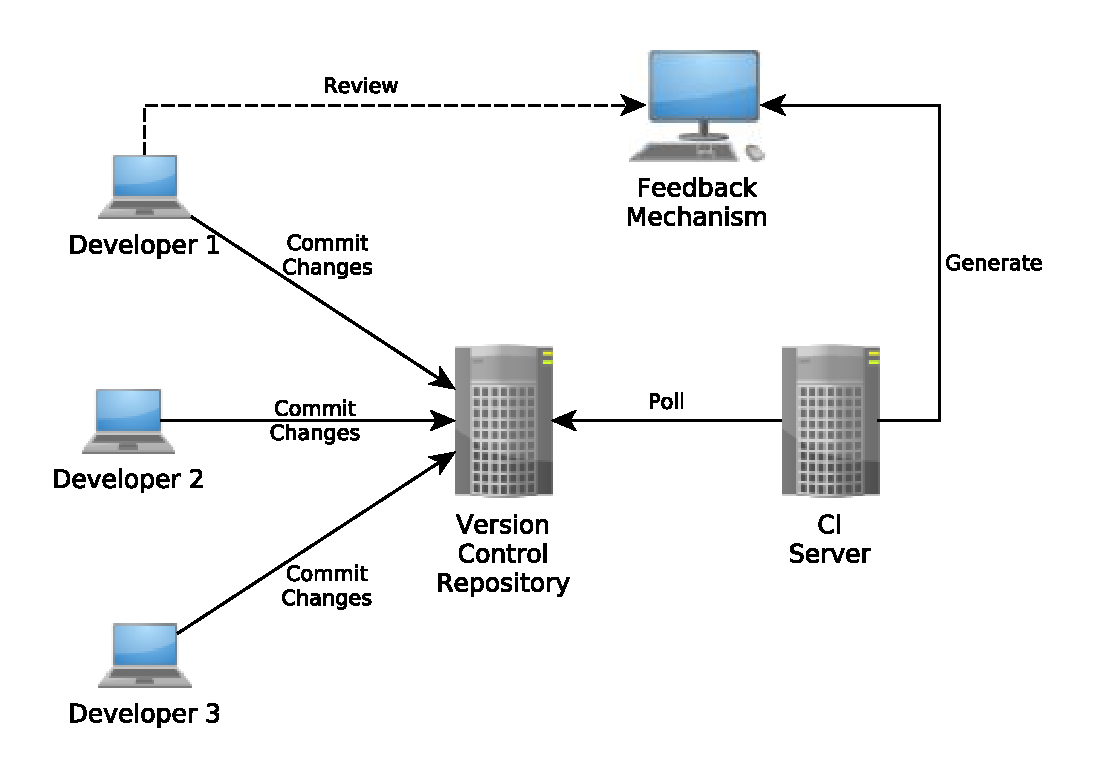
\includegraphics[scale=0.6]{yEd/components_of_CI_system.eps}
	\caption{Components of continuous integration system\cite{CIbook}}
	\label{fig:cocis}
\end{figure}

%=====================================================================================
\subsection{Demands of Continuous Integration}
%=====================================================================================

The minimal requirements for a good software development of a project where multiple developers are working on the same project are a version control repository and a continuous integration server. The version control system guarantees a software configuration management which is required for the continuous integration. The meaning of the version control system is very important. You cannot manage changes that developers had made in the source code without a version control system. The version control system has a very positive impact on the developing project. The system offers a history of changes which may be highly useful if a rollback is desired. Besides the history of changes, this system may save more other information about the source code, e.g. who did the change, when was the change created, etc. In addition, the version control system represents a primary source for the project source codes. This type of project setup is much more often used these days than in the past. Nearly every project has its own version control system which is provided by a repository hosting service.\\

A CI server has a huge advantage. This is a reason why it is highly recommended. It depends on the developer, how does he deploy the CI server. With the CI server, he does not have to bother with such many scripts for the automation. Nevertheless, as he decides how the CI server will be established, the system must contain these features. To facilitate the process of continuous integration, the system must support services as polling version control system, retention of build history, launching predefined steps such as scripts and tests. Furthermore, the system should offer an opportunity to send a feedback back to the developers. This server executes a series of actions or steps taken in order to achieve a particular end of CI. The next subsection will determine and state these fundamental steps of the continuous integration scenario and describe and illustrate them in detail.

%=====================================================================================
\subsection{Stages of Continuous Integration}
%=====================================================================================

The stages of CI insure code inspection and code integration. Before we begin, we need to clarify certain concepts which will be used later. To understand these steps, we need to understand what is the difference between \textbf{a build}, \textbf{a private build} and \textbf{an integration build}.

\begin{DEF}
A build may refer to a set of activities performed to generate, test, inspect, and deploy software\cite{CIbook}.
\end{DEF}

\begin{DEF}
A private build define a process in which a software developer runs the build on his local machine to ensure that the changes he made work before he commits them into a version control repository.
\end{DEF}

\begin{DEF}
An integration build is the act of combining software components (programs and files) into a software system\cite{CIbook}.
\end{DEF}

Now as we know what are these concepts we will illustrate the basic stages of continuous integration. To describe it properly, imagine that we have a group of developers working on the same project using a version control system where the source code of the software product is held, and they use a continuous integration service. The stages of continuous integration are the following:

\begin{enumerate}

	\item \textbf{The change}\\[0.1em]
		  One developer who wish to make a change, adjustment, improvement or to create a new feature in the software product has to clone the remote version control repository to his local computer to download the source code of the software product. At this point, he has a local version control repository in which he will do the changes he would like to. After a change is made, the change is only in a local repository and the developer would like to commit it into the remote repository. Before publishing the change, he has to run a private build. The developer has to publish the change he made which is a request for an approval of the change ready to merge into a specific branch on the remote repository. These not merged changes are published on the remote version of the control repository.\\[0.1em]
		  By committing changes to the version control repository a continuous integration server is invoked. The continuous integration server polles the version control repository when a change is detected, after this poll a reaction occures.

	\item \textbf{The reaction}\\[0.1em]
		  When a change is detected it invokes a continuous integration server to execute a few tasks. The tasks are predefined in a build script which has to integrate the change with the rest of the source code of the software product. The script provide source code compilation, database integration, testing and code inspection. The execution of the script is referred to as an integration build.\\[0.1em]
		  This stage of continuous integration usually includes also code verification. It finds defects or errors made by developer, e.g a compilation fail, tests failures etc. The errors are detected by tests which should have high code coverage. A number of errors in this stage can be reduced by launching a private build which may be less complex compared to launching the build script. Passing this stage depends on success of the build script which must be success on 100\%.

	\item \textbf{The feedback}\\[0.1em]
		  The continuous integration server generates a feedback associated to the results of the build which is assigned to this change and it might be sent to the author of the change. There is log information generated every time, by passing stage before, and it is held and assigned to the change. Feedback is given to the developer in a certain predefined form, e.g. email with failures only. The log file is saved on the continuous integration server where there is an overview about the builds and their stats.

	\item \textbf{The waiting}\\[0.1em]
		  This stage is the end of the process. It stands for continuous polling of  the version control repository waiting for a new change. Detecting a change will cause launching the stages from the beginning.

\end{enumerate}

%=====================================================================================
\subsection{Continuous Integration Server}
%=====================================================================================

If the software development proceed to use continuous integration in the workflow it might have a configured CI server. The principal sense of a continuous integration server is to get rid of a manual integration build. The configuration of the CI server depends on source code verification requirements and on type of polling. The CI server can also provide an additional automation for necessary essentials to the development such as integration, deployment, etc.\\

The continuous integration system is based on automation that is conducted by CI server. Automation is an act, when manual tasks are united and executed together in order to simplify the execution of manual tasks. Nowadays, in software development automations can be found in different parts of software development. It helps to accelerate the development process. In a CI system, there are different types of builds and mechanisms used for the automation.

\subsubsection{Polling}

We can distinguish several types of build mechanisms such as on-demand, scheduled, poll for change and event-driven mechanism\cite{CIbook}. The simplest automated mechanism, on-demand mechanism, can be done by single script in order to get rid of tasks repetition executed by the developer. The on-demand mechanism is an user-driven process in which someone manually initiates an integration build\cite{CIbook}. Scheduled mechanism is a planned event accomplished by CI server in predefined time. In the situation where multiple developers are frequently working on a product during the day, the best choice for a build should be a time planned in night. The scheduled type is used particularly when an advanced build of the software product is needed to be done. Scheduled processes are driven by time, for instance, so that it runs on an hourly basis, whether or not a change has occurred\cite{CIbook}.\\

Poll for change mechanism and event-driven mechanism differ only in a way of invoking. Poll for change mechanism uses a periodic time for a change polling and the event-driven mechanism is time independent mechanism which is invoked by a version control repository. In a poll for change mechanism, a process wakes up in a regular intervals and checks for changes to the version control repository, if changes are detected an integration build is ran\cite{CIbook}. The event-driven mechanism is triggered by a version control repository, if change was detected by version control repository than it initializes the build script. Only in these two mechanisms there is a polling service which is sectionalized into two different types.\\

Types of polling can be divided into two parts - time dependent polling and change dependent polling. The CI server with time dependent polling is configured to check the version control repository for a new change in predefined periodic time intervals e.g. every 10 minutes. Contrawise, the CI server with change dependent polling is invoked with every single action which is a change in a version control repository via an informative message about the current action sent to the CI server. This message including event stats is triggered on a specified event in the version control repository which must support this feature.\\

Time dependent polling is mostly used in general due to inadequacies such as missing event triggering in the version control repository. Due to this fundamental feature some of CI servers has to have  periodic polling on time. The main disadvantage is the time taken by downloading the actual source code from the repository. After the download is complete, the changes are still unknown, a comparison must be done between the latest and the last source code for the purpose of obtaining the new changes. Change dependent polling downloads only the real change towards the actual source code status made in the repository. If the version control system can support this feature the source code synchronization is much more faster and efficiently done.

%=====================================================================================
\subsection{Build Script}
%=====================================================================================

Instigation of CI system begin with a change in the version control system resulting in build script execution. Transforming sources into a system and simultaneously providing a review about the transformation is an intricate process also known as continuous integration, delivery and deployment. A CI system uses a build script allowing build automation, which includes every predestined statement to execute. This automation had a magnificent demand in software development. To get rid of constantly repeated actions for the purpose to accelerate the software development a build script was created. The principal script consists of a set of subscripts, which divide the automation into segments that are bound to themselves according to the execution order. Segments are shown in order in Figure \ref{fig:lpobs}. It shows the logical parts of a build script. Script performs a build also called as a software build which is not just about the source code compilation and tests launch. These various smoothly executed parts construct a functional unit of the software product. A working function unit congregation leads to working software deployment as the final step of CI. The script warrants simplification because of the developers adjust the source code and they are able to gain instant feedback about their work. As Martin Fowler said \uv{Get everything you need into source control get it so that you can build the whole system with a single command.}\cite{MartinFowler}.

\begin{figure}[H]
	\centering
	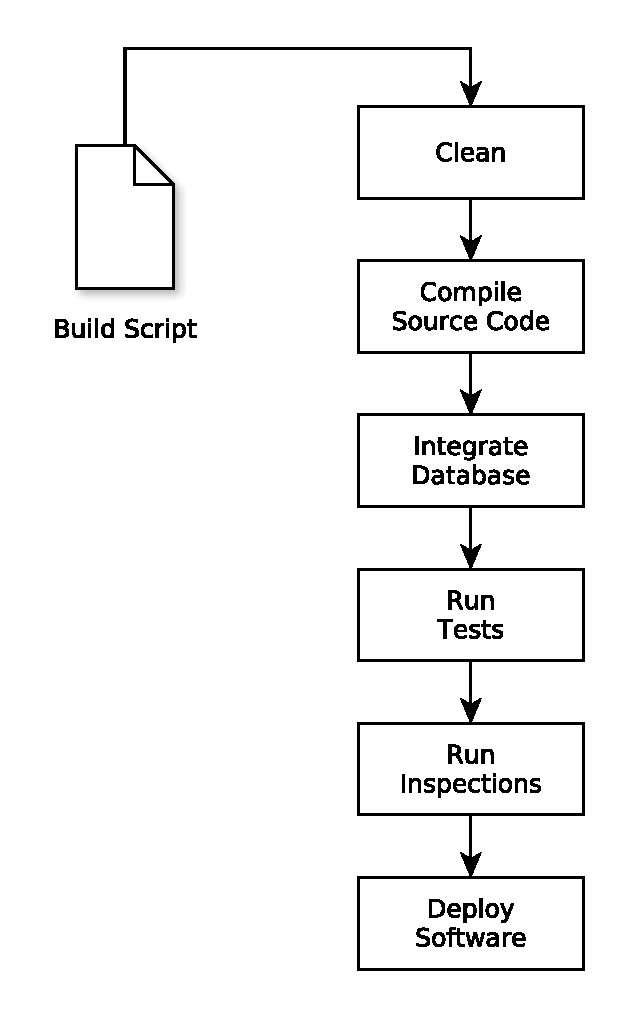
\includegraphics[scale=0.5]{yEd/the_logical_processes_of_a_build_script.eps}
	\caption{The logical processes of a build script\cite{CIbook}}
	\label{fig:lpobs}
\end{figure}

The whole point of continuous integration is to provide rapid feedback\cite{MartinFowler}. Developers would like to have as fast feedback as possible. To guarantee this quality there are different types of build scripts provided on different roles of requests. Build scripts are divided by the role as lightweight and heavyweight scripts. Lightweight scripts are much more faster than heavyweight scripts. They are used on principle of speed. To ensure this behavior, at first the lightweight scripts are initiated because they can easily catch the basic vulnerabilities and then more advanced tests, inspections, and others are launched by heavyweight scripts which leads to an integration build. Martin Fowler marked the lightweight script which does the first build, as a \uv{commit build}\cite{MartinFowler}. These scripts endeavor for quickness, error detection and software integration, besides that, they also provide a feedback about the results of the whole process to the developer.

\hfill\\
{\color{red}TODO: Build script and its parts description (shortly)}

%=====================================================================================
\subsection{Best Practices {\color{red}- maybe wrong section name TODO}}
%=====================================================================================

Continuous integration is a practice, not a tool\cite{CollabNet}. Martin Fowler on first of May 2006 stated the basics of CI and the best practices of CI in his article in which he remitted on still popularizing usage of CI. In addition to this article, there was a research provided by a group of scientists about the CI on project provided for the most part from GitHub. Their research is an empirical study about the usage, costs and benefits of CI which are concisely shown in abundant diagrams. The observation of CI and its usage pointed out the significant essential role of CI in open source projects. On the basis of the informations obtained from the researches about the CI, we can make a judgment that this practice will be more and more used in the open source projects. Thanks to automation and standardization, CI helps to effectively prevent errors when deploying applications into operation\cite{CIcure}.\\

Continuous Integration is also referred to as a \uv{cure for human error in deployment}\cite{CIcure} because of error prevention which is rapidly reduced by using this practice. The job of a developer includes a project build repetition which may be also reduced to a few of them for the sense of tasks rate reduction applied on developer. These processes leverage extensive automation and encourage constant code sharing to fix defects early\cite{DigitalOceanCI}. Many of errors, bugs, defects and vulnerabilities are reduced but not every of them is detected by using a CI, but nevertheless the manual software integration is excluded because of CI comprises it as the last step of the software deployment. The impact of the CI usage in software engineering will have extreme demand in the future of IT, more precisely in agile teams using extreme programming technique or any other agile technique. The usage of CI is very adaptive and versatile and it will be more and more used in forthcoming open source projects or any another projects which may not be open source only.\\

In general, if any group of developers would like to use a CI practice, they should fulfill few standards and dwell on these standards. In order for developers to benefit from implementing the practice of CI, they should change their typical day-to-day software development habits\cite{CIQualityFramework}. Usage of CI is beneficial sideline when a developer commits frequently, daily, often, probably few times per day. Farthest, the project should be hosted somewhere on any kid of version control repository which represents a main source for the source code of the product. Besides these two sole development requirements, the expectations are that the developers should not try to commit a broken code. It is avoidable by initiating a private build on their local machine, which decrease the fail chance of the build launched by the CI server.\\

By using CI practice, the risks as software corruption and integration problems are reduced appreciably and any kid of bugs are uncovered quickly. The integration may take unpredictable long time but the use of the CI practice resolve this problem by integrating the software frequently which may result in a few small kind of integration issues. Some other software methodologies integrate their work once after a long time which brings their software to face an incredibly huge integration problem. Martin Fowler pointed this problem in his article: \uv{I was told that this project had been in development for a couple of years and was currently integrating, and had been integrating for several months.}\cite{MartinFowler}. Several articles describe this long time integration as a \textit{Big Bang Integration}\cite{AaltoUniversity}. As we can see on Figure \ref{fig:integration} the risk of the software integration is markedly reduced by using a CI practice.

\hfill\\
{\color{red}GRAPH from \cite{AaltoUniversity} page 12/42 - continuous integration vs big bang integration}

\begin{figure}[H]
	\centering
	%\includegraphics[scale=1]{}
	\caption{Integration of the software.\cite{AaltoUniversity}}
	\label{fig:integration}
\end{figure}

Prevention against any type of error in a CI is solved via integration build performed on a CI server. Predicting the result of build has drawn the interest of academia and industry\cite{ResultsOfCIbuild}. Travis CI community has created a TravisTorrent\footnote{TravisTorrent was chosen to resemble the close proximity to the GHTorrent project\cite{TravisTorrentWEBPAGE}.}\cite{TravisTorrent} for the purpose of providing a huge amount of information about the builds for full-stack research on continuous integration which is still a developed prototype. Alongside the TravisTorrent, the GitHub company has provided information about the data inside of their version control system in a project called \uv{The GHTorrent project}\footnote{The name signifies a torrent of data coming from GitHub\cite{GHTorrentWEBPAGE}.}\cite{GHTorrent}. Based on these given informations as an open dataset, a few analysis were conducted on them resolving the CI practice in a real life developed projects. The best practices were established on the results of the empirical studies of these obtained data sets provided by many of companies.

%=====================================================================================
\subsubsection{Benefits of Continuous Integration}
%=====================================================================================

Asdf.


%=====================================================================================
\section{Code Review}
%=====================================================================================

{\color{red}TODO: types(manual / automated), (+)(-), vulnerabilities}

\subsection{Automated Code Review}

Asdf.

%=====================================================================================
\chapter{Continuous Integration in Open Source Projects}
%=====================================================================================

Asdf.

%=====================================================================================
\section{Open Source}
%=====================================================================================

Asdf.

%=====================================================================================
\section{Github}
%=====================================================================================

Asdf.

%=====================================================================================
\section{TravisCI}
%=====================================================================================

Asdf.

%=====================================================================================
\chapter{Conclusion}
%=====================================================================================

Asdf.
%a\cite{MIQBOT}, b\cite{GHMP}, c\cite{ThoughtWorks}
